In an initial approach, we are interested in knowing how well metrics fit our twelve category classification. To achieve this, we have executed two popular clustering algorithms which are going to group our set of elements (composed of the different style features) in such a way that members of the same group (called a cluster) are more similar in one way or another. These algorithms are K-Means \citep{hartigan1975clustering} and DBSCAN \citep{ester1996density}.

\begin{algorithm}
	\begin{algorithmic}[1]
		\REQUIRE Data set $X$ (represented as a matrix whose columns are the features and whose rows are the different samples) with missing values, number of clusters $k$ and the maximum number of iterations to perform $maxiter$.
		\ENSURE A vector $labels$ that indicates to which cluster each element belongs and a data set $X^\prime$ which is a copy of $X$ with the missing values filled in.
		\STATE $X^\prime = X$
		\STATE $missing = $ list of positions (pair of rows and columns) of the missing values of $X$
		\FOR {$(row, column)$ in $missing$}
		\STATE $X^\prime[row, column] = mean(X[, column])$
		\ENDFOR
		\STATE $i = 1$
		\STATE $converge =$ \FALSE
		\STATE $prevlabels, prevcentroids = KMeans(init = random, k, X^\prime)$
		\FOR {$(row, column)$ in $missing$}
		\STATE $X^\prime[row, column] = prevcentroids[prevlabels[row]][column]$
		\ENDFOR
		\WHILE {$i < maxiter$ $\land$ $\lnot converge$}
		\STATE $labels, centroids = KMeans(init = prevlabels, k, X^\prime)$
		\FOR {$(row, column)$ in $missing$}
		\STATE $X^\prime[row, column] = centroids[labels[row]][column]$
		\ENDFOR
		\STATE $converge =$ $(prevlabels == labels)$
		\IF{$\lnot converge$}
		\STATE $prevlabels = labels$
		\STATE $prevcentroids = centroids$
		\STATE $i = i + 1$
		\ENDIF
		\ENDWHILE
		\RETURN $labels, X^\prime$
	\end{algorithmic}
	\caption{K-Means with missing values}\label{alg:kpod}
\end{algorithm}

Both algorithms require a parameter (in the case of K-Means the parameter is the number of clusters and in the case of DBSCAN the threshold distance that determines a neighbourhood of elements) which has to be defined before their execution. To make the decision of the initial value of the parameter there are methods based on the internal and cluster dispersion obtained. For this purpose, measures are taken to help the decision, such as the Silhouette Coefficient \citep{rousseeuw1987silhouettes}. It is a method of interpretation and validation of consistency within clusters of data. The technique provides a succinct graphical representation of how well each object has been classified. The best value is 1 and the worst value is -1. Values near 0 indicate overlapping clusters. Negative values generally indicate that a sample has been assigned to the wrong cluster, as a different cluster is more similar. Likewise, we can obtain a general idea of the behaviour of the clustering by calculating the mean Silhouette Coefficient for all samples.

Furthermore, we need to assess how much our classification resembles the clusters obtained after the execution of each of the algorithms. For this evaluation, we can use the Adjusted Rand Index (ARI), which is a form of the Rand index \citep{rand1971objective} that conforms to the random grouping of elements. The Adjusted Rand index is thus ensured to have a value close to 0.0 for random labelling independently of the number of clusters and samples and exactly 1.0 when the clusterings are identical (up to a permutation).

Due to the presence of NaN values, we are not able to use the K-Means algorithm directly on the data. Instead of replacing the NaN values as we have explained in Section \ref{sect:DatPrep}, we are going to use a slight variation from the K-POD algorithm \citep{chi2016k}, which runs K-Means iteratively while it modifies the cells where the value is missing by assigning the value of the centroids. The algorithm that we are going to use, similar to the K-POD, is the one shown in Algorithm \ref{alg:kpod}, where we have two invoked functions. The first one is \textit{mean}, which returns the mean of the given array without taking into account the missing values. The second one, \textit{KMeans}, is a function that applies the K-Means algorithm given a set of initial centroids (or it will generate them randomly), the number of clusters and the dataset. It returns an array as long as the number of rows of the given dataset which indicates the cluster index (through an integer) that each element belongs to and the coordinates (features values) of the centroid of each cluster (it will be a matrix with as many rows as the number of cluster and as many columns as the numbers of features).

Now that we have chosen the algorithm, we execute it with different $k$ parameter (the number of clusters). The rest of the input will be the normalised data with the NaN values and with a maximum of 100 iteration. With each $k$-dependent execution, we will calculate the Silhouette Score (which is the mean of the Silhouette Coefficient of all samples) and the Adjusted Rand Index given the real classification. As a result of this we obtain Figures \ref{fig:nkmeanssil} and \ref{fig:nkmeansari}.

\begin{figure}
	\begin{minipage}[b]{0.37\paperwidth}
	\centerline{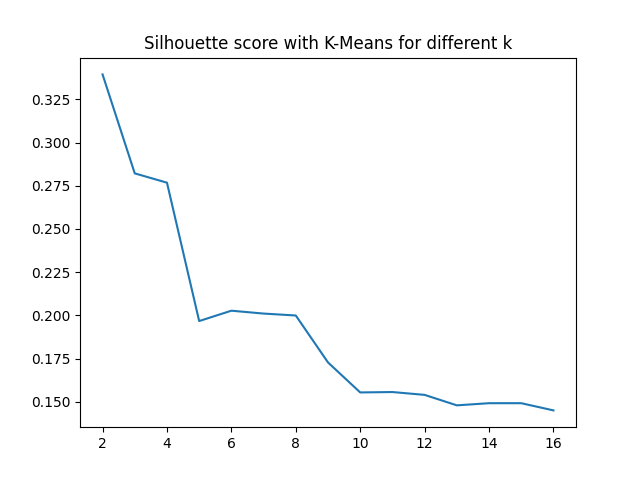
\includegraphics[width=\textwidth]{Imagenes/Bitmap/Clustering/normkmeanssil.png}}%
	\caption{Silhouette Score with K-Mean}%
	\label{fig:nkmeanssil}
	\end{minipage}
	\begin{minipage}[b]{0.37\paperwidth}
		\centerline{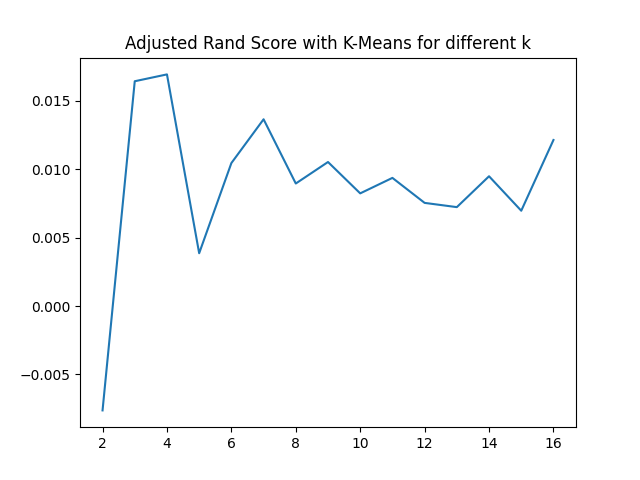
\includegraphics[width=\textwidth]{Imagenes/Bitmap/Clustering/normkmeansrand.png}}%
		\caption{ARI with K-Means}%
		\label{fig:nkmeansari}
	\end{minipage}
\end{figure}

In respect of the Silhouette Score analysis (which is shown in Figure \ref{fig:nkmeanssil}), with the given values, we are able to claim that, in general, as the number of groups increases the Silhouette Score decreases. This fact indicates us that the best number of clusters in order to achieve a good differentiation between each group of elements is two, which is not in line with our classification model. Not surprisingly, these results, which do not fit well in the established categories, are accompanied by poor values of the Adjusted Rand Index. As we can observe in Figure \ref{fig:nkmeansari}, all the obtained values with any number of cluster is very close to zero, which means, as we have previously explained, that the obtained classification does not match with ours.

In the case of DBSCAN algorithm, we are going to replace the missing values as we have explained in Section \ref{sect:DatPrep}. This clustering technique needs two different parameters: the threshold distance that determines a neighbourhood of elements (denoted by $\varepsilon$) and the minimum number of elements that forms a cluster. We will assign the value of three to this last parameter. This choice is motivated by the distribution between the different categories that we have previously defined. As we can observe in Figure \ref{fig:distr}, the smallest class has three elements in it, so it would not be consistent with our classification if a minimum number bigger than three is established. Moreover, the value of one does not make sense, since all the points of your data set will be a cluster (we would lose the possibility of detecting noise which is one of the advantages of DBSCAN over K-Means), and with 2 the result will be the same as the hierarchical cluster \citep{nielsen2016hierarchical} with the single-link metric, with the cut at the height of the dendrogram $\varepsilon$.

As we have done with K-Means, we are going to execute the DBSCAN algorithm with different $\varepsilon$ parameters. Besides, both the euclidean and manhattan metric are going to be used for this analysis. However, we will get similar results in both cases, so we are going to present the values obtained with the euclidean metric (see Figure \ref{fig:dbscaneu}).

\begin{figure}[t]
	\centering%
	\centerline{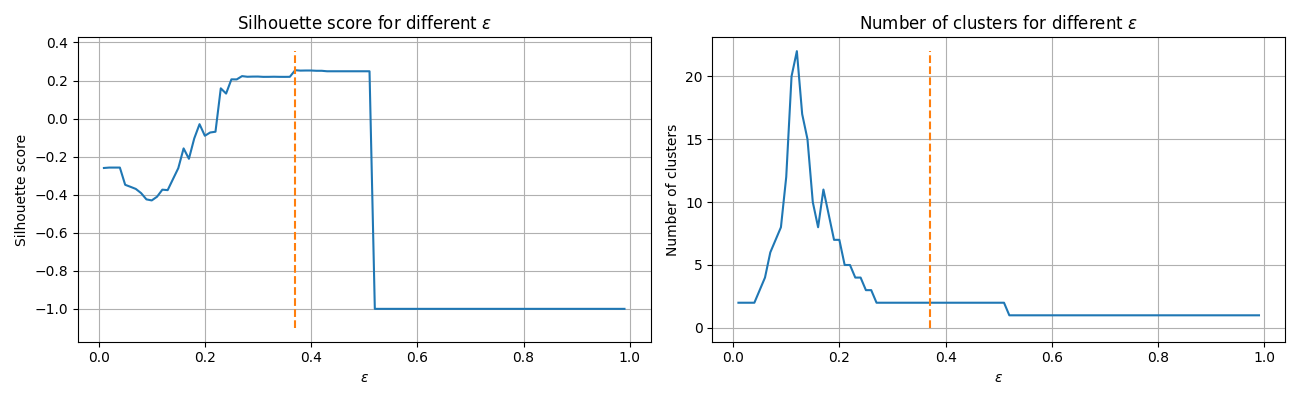
\includegraphics[width=\textwidth]{Imagenes/Bitmap/Clustering/dbscansil.png}}%
	\caption{Results of DBSCAN execution with euclidean metric}%
	\label{fig:dbscaneu}
\end{figure}

As in the case of the K-Means algorithm, we can find the maximum Silhouette Score with two clusters, which is not in line with our classification model. Furthermore, as we can see in Figure \ref{fig:dbscanari}, we find again values very close to zero in the Adjusted Rand Index analysis.

In conclusion, using the clustering techniques to classify the messages according to the selected metrics, as expected, we do not obtain significant results that fit our model or allow us to group the different e-mails in another way. One of the problems found to achieve this is the great amount of states that each element has, that is, the high number of dimensions of the system. We also find this inconvenience when we try to get the main statistics of the different features that describe the messages. Therefore, it is an issue that must be addressed (the reduction of dimensionality), especially trying that this reduction serves to adapt to the categorization carried out or to obtain a smaller number of parameters that define the writing style.

\begin{figure}[h]
	\centering%
	\centerline{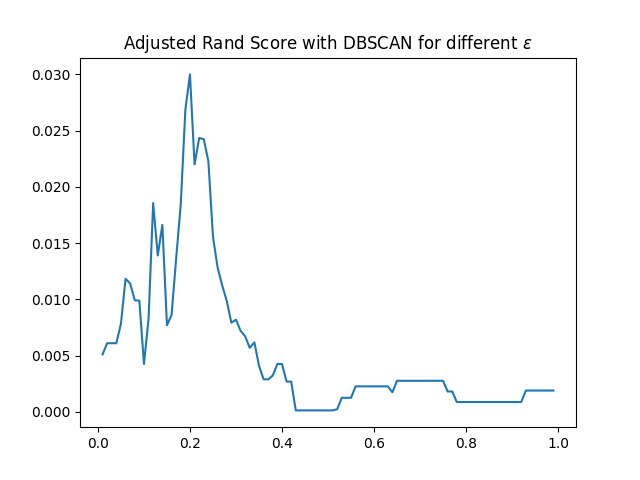
\includegraphics[width=0.5\textwidth]{Imagenes/Bitmap/Clustering/dbscanari.png}}%
	\caption{Adjusted Rand Index of DBSCAN with euclidean metric}%
	\label{fig:dbscanari}
\end{figure}